\documentclass[twoside]{book}

% Packages required by doxygen
\usepackage{fixltx2e}
\usepackage{calc}
\usepackage{doxygen}
\usepackage[export]{adjustbox} % also loads graphicx
\usepackage{graphicx}
\usepackage[utf8]{inputenc}
\usepackage{makeidx}
\usepackage{multicol}
\usepackage{multirow}
\PassOptionsToPackage{warn}{textcomp}
\usepackage{textcomp}
\usepackage[nointegrals]{wasysym}
\usepackage[table]{xcolor}

% Font selection
\usepackage[T1]{fontenc}
\usepackage[scaled=.90]{helvet}
\usepackage{courier}
\usepackage{amssymb}
\usepackage{sectsty}
\renewcommand{\familydefault}{\sfdefault}
\allsectionsfont{%
  \fontseries{bc}\selectfont%
  \color{darkgray}%
}
\renewcommand{\DoxyLabelFont}{%
  \fontseries{bc}\selectfont%
  \color{darkgray}%
}
\newcommand{\+}{\discretionary{\mbox{\scriptsize$\hookleftarrow$}}{}{}}

% Page & text layout
\usepackage{geometry}
\geometry{%
  a4paper,%
  top=2.5cm,%
  bottom=2.5cm,%
  left=2.5cm,%
  right=2.5cm%
}
\tolerance=750
\hfuzz=15pt
\hbadness=750
\setlength{\emergencystretch}{15pt}
\setlength{\parindent}{0cm}
\setlength{\parskip}{3ex plus 2ex minus 2ex}
\makeatletter
\renewcommand{\paragraph}{%
  \@startsection{paragraph}{4}{0ex}{-1.0ex}{1.0ex}{%
    \normalfont\normalsize\bfseries\SS@parafont%
  }%
}
\renewcommand{\subparagraph}{%
  \@startsection{subparagraph}{5}{0ex}{-1.0ex}{1.0ex}{%
    \normalfont\normalsize\bfseries\SS@subparafont%
  }%
}
\makeatother

% Headers & footers
\usepackage{fancyhdr}
\pagestyle{fancyplain}
\fancyhead[LE]{\fancyplain{}{\bfseries\thepage}}
\fancyhead[CE]{\fancyplain{}{}}
\fancyhead[RE]{\fancyplain{}{\bfseries\leftmark}}
\fancyhead[LO]{\fancyplain{}{\bfseries\rightmark}}
\fancyhead[CO]{\fancyplain{}{}}
\fancyhead[RO]{\fancyplain{}{\bfseries\thepage}}
\fancyfoot[LE]{\fancyplain{}{}}
\fancyfoot[CE]{\fancyplain{}{}}
\fancyfoot[RE]{\fancyplain{}{\bfseries\scriptsize Generated by Doxygen }}
\fancyfoot[LO]{\fancyplain{}{\bfseries\scriptsize Generated by Doxygen }}
\fancyfoot[CO]{\fancyplain{}{}}
\fancyfoot[RO]{\fancyplain{}{}}
\renewcommand{\footrulewidth}{0.4pt}
\renewcommand{\chaptermark}[1]{%
  \markboth{#1}{}%
}
\renewcommand{\sectionmark}[1]{%
  \markright{\thesection\ #1}%
}

% Indices & bibliography
\usepackage{natbib}
\usepackage[titles]{tocloft}
\setcounter{tocdepth}{3}
\setcounter{secnumdepth}{5}
\makeindex

% Hyperlinks (required, but should be loaded last)
\usepackage{ifpdf}
\ifpdf
  \usepackage[pdftex,pagebackref=true]{hyperref}
\else
  \usepackage[ps2pdf,pagebackref=true]{hyperref}
\fi
\hypersetup{%
  colorlinks=true,%
  linkcolor=blue,%
  citecolor=blue,%
  unicode%
}

% Custom commands
\newcommand{\clearemptydoublepage}{%
  \newpage{\pagestyle{empty}\cleardoublepage}%
}

\usepackage{caption}
\captionsetup{labelsep=space,justification=centering,font={bf},singlelinecheck=off,skip=4pt,position=top}

%===== C O N T E N T S =====

\begin{document}

% Titlepage & ToC
\hypersetup{pageanchor=false,
             bookmarksnumbered=true,
             pdfencoding=unicode
            }
\pagenumbering{roman}
\begin{titlepage}
\vspace*{7cm}
\begin{center}%
{\Large Final experimental assignment }\\
\vspace*{1cm}
{\large Generated by Doxygen 1.8.11}\\
\end{center}
\end{titlepage}
\clearemptydoublepage
\tableofcontents
\clearemptydoublepage
\pagenumbering{arabic}
\hypersetup{pageanchor=true}

%--- Begin generated contents ---
\chapter{slam\+\_\+gmapping}
\label{index}\hypertarget{index}{} {\bfseries slam\+\_\+gmapping} is a wrapper around the G\+Mapping S\+L\+AM library. It reads laser scans and odometry and computes a map. This map can be written to a file using e.\+g. \char`\"{}rosrun map\+\_\+server map\+\_\+saver static\+\_\+map\+:=dynamic\+\_\+map\char`\"{} 

 \hypertarget{index_topic}{}\section{R\+O\+S topics}\label{index_topic}
Subscribes to (name/type)\+:
\begin{DoxyItemize}
\item {\bfseries \char`\"{}scan\char`\"{}/} \href{../../sensor_msgs/html/classstd__msgs_1_1LaserScan.html}{\tt sensor\+\_\+msgs/\+Laser\+Scan} \+: data from a laser range scanner
\item {\bfseries \char`\"{}/tf\char`\"{}}\+: odometry from the robot Publishes to (name/type)\+:
\item {\bfseries \char`\"{}/tf\char`\"{}/tf/tf\+Message}\+: position relative to the map 
\end{DoxyItemize}\hypertarget{index_services}{}\section{services}\label{index_services}

\begin{DoxyItemize}
\item {\bfseries \char`\"{}$\sim$dynamic\+\_\+map\char`\"{}} \+: returns the map 
\end{DoxyItemize}\hypertarget{index_parameters}{}\section{R\+O\+S parameters}\label{index_parameters}
Reads the following parameters from the parameter server Parameters used by our G\+Mapping wrapper\+:
\begin{DoxyItemize}
\item {\bfseries \char`\"{}$\sim$throttle\+\_\+scans\char`\"{}}\+: {\bfseries }\mbox{[}int\mbox{]} throw away every nth laser scan
\item {\bfseries \char`\"{}$\sim$base\+\_\+frame\char`\"{}}\+: {\bfseries }\mbox{[}string\mbox{]} the tf frame\+\_\+id to use for the robot base pose
\item {\bfseries \char`\"{}$\sim$map\+\_\+frame\char`\"{}}\+: {\bfseries }\mbox{[}string\mbox{]} the tf frame\+\_\+id where the robot pose on the map is published
\item {\bfseries \char`\"{}$\sim$odom\+\_\+frame\char`\"{}}\+: {\bfseries }\mbox{[}string\mbox{]} the tf frame\+\_\+id from which odometry is read
\item {\bfseries \char`\"{}$\sim$map\+\_\+update\+\_\+interval\char`\"{}}\+: {\bfseries }\mbox{[}double\mbox{]} time in seconds between two recalculations of the map Parameters used by G\+Mapping itself\+: Laser Parameters\+:
\item {\bfseries \char`\"{}$\sim$/max\+Range\char`\"{}} {\bfseries }\mbox{[}double\mbox{]} maximum range of the laser scans. Rays beyond this range get discarded completely. (default\+: maximum laser range minus 1 cm, as received in the the first Laser\+Scan message)
\item {\bfseries \char`\"{}$\sim$/max\+Urange\char`\"{}} {\bfseries }\mbox{[}double\mbox{]} maximum range of the laser scanner that is used for map building (default\+: same as max\+Range)
\item {\bfseries \char`\"{}$\sim$/sigma\char`\"{}} {\bfseries }\mbox{[}double\mbox{]} standard deviation for the scan matching process (cell)
\item {\bfseries \char`\"{}$\sim$/kernel\+Size\char`\"{}} {\bfseries }\mbox{[}int\mbox{]} search window for the scan matching process
\item {\bfseries \char`\"{}$\sim$/lstep\char`\"{}} {\bfseries }\mbox{[}double\mbox{]} initial search step for scan matching (linear)
\item {\bfseries \char`\"{}$\sim$/astep\char`\"{}} {\bfseries }\mbox{[}double\mbox{]} initial search step for scan matching (angular)
\item {\bfseries \char`\"{}$\sim$/iterations\char`\"{}} {\bfseries }\mbox{[}int\mbox{]} number of refinement steps in the scan matching. The final \char`\"{}precision\char`\"{} for the match is lstep$\ast$2$^\wedge$(-\/iterations) or astep$\ast$2$^\wedge$(-\/iterations), respectively.
\item {\bfseries \char`\"{}$\sim$/lsigma\char`\"{}} {\bfseries }\mbox{[}double\mbox{]} standard deviation for the scan matching process (single laser beam)
\item {\bfseries \char`\"{}$\sim$/ogain\char`\"{}} {\bfseries }\mbox{[}double\mbox{]} gain for smoothing the likelihood
\item {\bfseries \char`\"{}$\sim$/lskip\char`\"{}} {\bfseries }\mbox{[}int\mbox{]} take only every (n+1)th laser ray for computing a match (0 = take all rays)
\item {\bfseries \char`\"{}$\sim$/minimum\+Score\char`\"{}} {\bfseries }\mbox{[}double\mbox{]} minimum score for considering the outcome of the scanmatching good. Can avoid \textquotesingle{}jumping\textquotesingle{} pose estimates in large open spaces when using laser scanners with limited range (e.\+g. 5m). (0 = default. Scores go up to 600+, try 50 for example when experiencing \textquotesingle{}jumping\textquotesingle{} estimate issues) Motion Model Parameters (all standard deviations of a gaussian noise model)
\item {\bfseries \char`\"{}$\sim$/srr\char`\"{}} {\bfseries }\mbox{[}double\mbox{]} linear noise component (x and y)
\item {\bfseries \char`\"{}$\sim$/stt\char`\"{}} {\bfseries }\mbox{[}double\mbox{]} angular noise component (theta)
\item {\bfseries \char`\"{}$\sim$/srt\char`\"{}} {\bfseries }\mbox{[}double\mbox{]} linear -\/$>$ angular noise component
\item {\bfseries \char`\"{}$\sim$/str\char`\"{}} {\bfseries }\mbox{[}double\mbox{]} angular -\/$>$ linear noise component Others\+:
\item {\bfseries \char`\"{}$\sim$/linear\+Update\char`\"{}} {\bfseries }\mbox{[}double\mbox{]} the robot only processes new measurements if the robot has moved at least this many meters
\item {\bfseries \char`\"{}$\sim$/angular\+Update\char`\"{}} {\bfseries }\mbox{[}double\mbox{]} the robot only processes new measurements if the robot has turned at least this many rads
\item {\bfseries \char`\"{}$\sim$/resample\+Threshold\char`\"{}} {\bfseries }\mbox{[}double\mbox{]} threshold at which the particles get resampled. Higher means more frequent resampling.
\item {\bfseries \char`\"{}$\sim$/particles\char`\"{}} {\bfseries }\mbox{[}int\mbox{]} (fixed) number of particles. Each particle represents a possible trajectory that the robot has traveled Likelihood sampling (used in scan matching)
\item {\bfseries \char`\"{}$\sim$/llsamplerange\char`\"{}} {\bfseries }\mbox{[}double\mbox{]} linear range
\item {\bfseries \char`\"{}$\sim$/lasamplerange\char`\"{}} {\bfseries }\mbox{[}double\mbox{]} linear step size
\item {\bfseries \char`\"{}$\sim$/llsamplestep\char`\"{}} {\bfseries }\mbox{[}double\mbox{]} linear range
\item {\bfseries \char`\"{}$\sim$/lasamplestep\char`\"{}} {\bfseries }\mbox{[}double\mbox{]} angular step size Initial map dimensions and resolution\+:
\item {\bfseries \char`\"{}$\sim$/xmin\char`\"{}} {\bfseries }\mbox{[}double\mbox{]} minimum x position in the map \mbox{[}m\mbox{]}
\item {\bfseries \char`\"{}$\sim$/ymin\char`\"{}} {\bfseries }\mbox{[}double\mbox{]} minimum y position in the map \mbox{[}m\mbox{]}
\item {\bfseries \char`\"{}$\sim$/xmax\char`\"{}} {\bfseries }\mbox{[}double\mbox{]} maximum x position in the map \mbox{[}m\mbox{]}
\item {\bfseries \char`\"{}$\sim$/ymax\char`\"{}} {\bfseries }\mbox{[}double\mbox{]} maximum y position in the map \mbox{[}m\mbox{]}
\item {\bfseries \char`\"{}$\sim$/delta\char`\"{}} {\bfseries }\mbox{[}double\mbox{]} size of one pixel \mbox{[}m\mbox{]} 
\end{DoxyItemize}
\chapter{Hierarchical Index}
\section{Class Hierarchy}
This inheritance list is sorted roughly, but not completely, alphabetically\+:\begin{DoxyCompactList}
\item \contentsline{section}{Perception.\+image\+\_\+feature}{\pageref{classPerception_1_1image__feature}}{}
\item Nodelet\begin{DoxyCompactList}
\item \contentsline{section}{Slam\+G\+Mapping\+Nodelet}{\pageref{classSlamGMappingNodelet}}{}
\end{DoxyCompactList}
\item State\begin{DoxyCompactList}
\item \contentsline{section}{Behaviors.\+Find}{\pageref{classBehaviors_1_1Find}}{}
\item \contentsline{section}{Behaviors.\+Normal}{\pageref{classBehaviors_1_1Normal}}{}
\item \contentsline{section}{Behaviors.\+Play}{\pageref{classBehaviors_1_1Play}}{}
\item \contentsline{section}{Behaviors.\+Recovery}{\pageref{classBehaviors_1_1Recovery}}{}
\item \contentsline{section}{Behaviors.\+Sleep}{\pageref{classBehaviors_1_1Sleep}}{}
\item \contentsline{section}{Behaviors.\+Track}{\pageref{classBehaviors_1_1Track}}{}
\end{DoxyCompactList}
\end{DoxyCompactList}

\chapter{Class Index}
\section{Class List}
Here are the classes, structs, unions and interfaces with brief descriptions\+:\begin{DoxyCompactList}
\item\contentsline{section}{\hyperlink{classexplore_1_1Costmap2DClient}{explore\+::\+Costmap2\+D\+Client} }{\pageref{classexplore_1_1Costmap2DClient}}{}
\item\contentsline{section}{\hyperlink{classexplore_1_1Explore}{explore\+::\+Explore} \\*A class adhering to the robot\+\_\+actions\+::\+Action interface that moves the robot base to explore its environment }{\pageref{classexplore_1_1Explore}}{}
\item\contentsline{section}{\hyperlink{classBehaviors_1_1Find}{Behaviors.\+Find} \\*\hyperlink{classBehaviors_1_1Find}{Find}\+: class that describes the \hyperlink{classBehaviors_1_1Find}{Find} state }{\pageref{classBehaviors_1_1Find}}{}
\item\contentsline{section}{\hyperlink{structfrontier__exploration_1_1Frontier}{frontier\+\_\+exploration\+::\+Frontier} \\*Represents a frontier }{\pageref{structfrontier__exploration_1_1Frontier}}{}
\item\contentsline{section}{\hyperlink{classfrontier__exploration_1_1FrontierSearch}{frontier\+\_\+exploration\+::\+Frontier\+Search} \\*Thread-\/safe implementation of a frontier-\/search task for an input costmap }{\pageref{classfrontier__exploration_1_1FrontierSearch}}{}
\item\contentsline{section}{\hyperlink{classPerception_1_1image__feature}{Perception.\+image\+\_\+feature} \\*C\+L\+A\+SS }{\pageref{classPerception_1_1image__feature}}{}
\item\contentsline{section}{\hyperlink{classBehaviors_1_1Normal}{Behaviors.\+Normal} \\*\hyperlink{classBehaviors_1_1Normal}{Normal}\+: class that describes the \hyperlink{classBehaviors_1_1Normal}{Normal} state }{\pageref{classBehaviors_1_1Normal}}{}
\item\contentsline{section}{\hyperlink{classBehaviors_1_1Play}{Behaviors.\+Play} \\*\hyperlink{classBehaviors_1_1Play}{Play}\+: class that describes the \hyperlink{classBehaviors_1_1Play}{Play} state }{\pageref{classBehaviors_1_1Play}}{}
\item\contentsline{section}{\hyperlink{classBehaviors_1_1Recovery}{Behaviors.\+Recovery} \\*\hyperlink{classBehaviors_1_1Recovery}{Recovery}\+: class that describes the \hyperlink{classBehaviors_1_1Recovery}{Recovery} state }{\pageref{classBehaviors_1_1Recovery}}{}
\item\contentsline{section}{\hyperlink{classSlamGMapping}{Slam\+G\+Mapping} }{\pageref{classSlamGMapping}}{}
\item\contentsline{section}{\hyperlink{classSlamGMappingNodelet}{Slam\+G\+Mapping\+Nodelet} }{\pageref{classSlamGMappingNodelet}}{}
\item\contentsline{section}{\hyperlink{classBehaviors_1_1Sleep}{Behaviors.\+Sleep} \\*\hyperlink{classBehaviors_1_1Sleep}{Sleep}\+: class that describes the \hyperlink{classBehaviors_1_1Sleep}{Sleep} state }{\pageref{classBehaviors_1_1Sleep}}{}
\item\contentsline{section}{\hyperlink{classBehaviors_1_1Track}{Behaviors.\+Track} \\*\hyperlink{classBehaviors_1_1Track}{Track}\+: class that describes the \hyperlink{classBehaviors_1_1Track}{Track} state }{\pageref{classBehaviors_1_1Track}}{}
\end{DoxyCompactList}

\chapter{Class Documentation}
\hypertarget{classBehaviors_1_1Find}{}\section{Behaviors.\+Find Class Reference}
\label{classBehaviors_1_1Find}\index{Behaviors.\+Find@{Behaviors.\+Find}}


\hyperlink{classBehaviors_1_1Find}{Find}\+: class that describes the \hyperlink{classBehaviors_1_1Find}{Find} state.  




Inheritance diagram for Behaviors.\+Find\+:\nopagebreak
\begin{figure}[H]
\begin{center}
\leavevmode
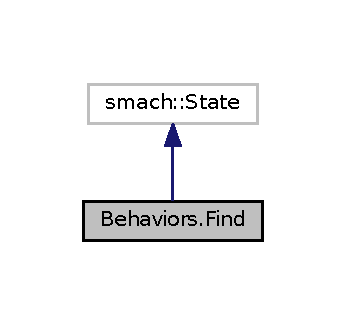
\includegraphics[width=166pt]{classBehaviors_1_1Find__inherit__graph}
\end{center}
\end{figure}


Collaboration diagram for Behaviors.\+Find\+:\nopagebreak
\begin{figure}[H]
\begin{center}
\leavevmode
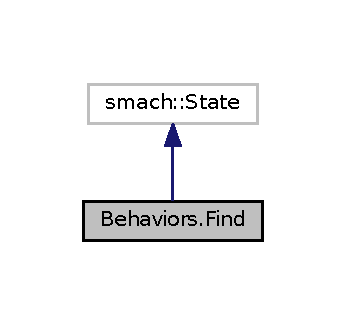
\includegraphics[width=166pt]{classBehaviors_1_1Find__coll__graph}
\end{center}
\end{figure}
\subsection*{Public Member Functions}
\begin{DoxyCompactItemize}
\item 
def {\bfseries \+\_\+\+\_\+init\+\_\+\+\_\+} (self)\hypertarget{classBehaviors_1_1Find_a50fe385da0196f85d03c9215531e8468}{}\label{classBehaviors_1_1Find_a50fe385da0196f85d03c9215531e8468}

\item 
def {\bfseries execute} (self, userdata)\hypertarget{classBehaviors_1_1Find_a4910773265944430bb02fc53318fb956}{}\label{classBehaviors_1_1Find_a4910773265944430bb02fc53318fb956}

\end{DoxyCompactItemize}


\subsection{Detailed Description}
\hyperlink{classBehaviors_1_1Find}{Find}\+: class that describes the \hyperlink{classBehaviors_1_1Find}{Find} state. 

The documentation for this class was generated from the following file\+:\begin{DoxyCompactItemize}
\item 
exp\+\_\+assignment3/scripts/Behaviors.\+py\end{DoxyCompactItemize}

\hypertarget{classPerception_1_1image__feature}{}\section{Perception.\+image\+\_\+feature Class Reference}
\label{classPerception_1_1image__feature}\index{Perception.\+image\+\_\+feature@{Perception.\+image\+\_\+feature}}


C\+L\+A\+SS.  


\subsection*{Public Member Functions}
\begin{DoxyCompactItemize}
\item 
def \hyperlink{classPerception_1_1image__feature_a748b3574bea982b0e5b29a86dfca644e}{\+\_\+\+\_\+init\+\_\+\+\_\+} (self)
\item 
def {\bfseries callback} (self, ros\+\_\+data)\hypertarget{classPerception_1_1image__feature_aa4163f3a9600d001cfd6ac90ba460df9}{}\label{classPerception_1_1image__feature_aa4163f3a9600d001cfd6ac90ba460df9}

\end{DoxyCompactItemize}
\subsection*{Public Attributes}
\begin{DoxyCompactItemize}
\item 
{\bfseries image\+\_\+pub}\hypertarget{classPerception_1_1image__feature_acfc602315032d7e877533594d93ed051}{}\label{classPerception_1_1image__feature_acfc602315032d7e877533594d93ed051}

\item 
{\bfseries vel\+\_\+pub}\hypertarget{classPerception_1_1image__feature_a2582bcb9aca24ef19e5a249684048c84}{}\label{classPerception_1_1image__feature_a2582bcb9aca24ef19e5a249684048c84}

\item 
{\bfseries subscriber}\hypertarget{classPerception_1_1image__feature_a73606194793aca7799100ae95535b072}{}\label{classPerception_1_1image__feature_a73606194793aca7799100ae95535b072}

\end{DoxyCompactItemize}


\subsection{Detailed Description}
C\+L\+A\+SS. 

Image feature class to handle feature identification inside the image sent by the camera 

\subsection{Constructor \& Destructor Documentation}
\index{Perception\+::image\+\_\+feature@{Perception\+::image\+\_\+feature}!\+\_\+\+\_\+init\+\_\+\+\_\+@{\+\_\+\+\_\+init\+\_\+\+\_\+}}
\index{\+\_\+\+\_\+init\+\_\+\+\_\+@{\+\_\+\+\_\+init\+\_\+\+\_\+}!Perception\+::image\+\_\+feature@{Perception\+::image\+\_\+feature}}
\subsubsection[{\texorpdfstring{\+\_\+\+\_\+init\+\_\+\+\_\+(self)}{__init__(self)}}]{\setlength{\rightskip}{0pt plus 5cm}def Perception.\+image\+\_\+feature.\+\_\+\+\_\+init\+\_\+\+\_\+ (
\begin{DoxyParamCaption}
\item[{}]{self}
\end{DoxyParamCaption}
)}\hypertarget{classPerception_1_1image__feature_a748b3574bea982b0e5b29a86dfca644e}{}\label{classPerception_1_1image__feature_a748b3574bea982b0e5b29a86dfca644e}
\begin{DoxyVerb}Initialize ros publisher, ros subscriber\end{DoxyVerb}
 

The documentation for this class was generated from the following file\+:\begin{DoxyCompactItemize}
\item 
exp\+\_\+assignment3/scripts/Perception.\+py\end{DoxyCompactItemize}

\hypertarget{classBehaviors_1_1Normal}{}\section{Behaviors.\+Normal Class Reference}
\label{classBehaviors_1_1Normal}\index{Behaviors.\+Normal@{Behaviors.\+Normal}}


\hyperlink{classBehaviors_1_1Normal}{Normal}\+: class that describes the \hyperlink{classBehaviors_1_1Normal}{Normal} state.  




Inheritance diagram for Behaviors.\+Normal\+:\nopagebreak
\begin{figure}[H]
\begin{center}
\leavevmode
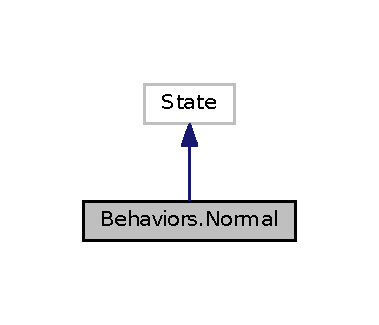
\includegraphics[width=182pt]{classBehaviors_1_1Normal__inherit__graph}
\end{center}
\end{figure}


Collaboration diagram for Behaviors.\+Normal\+:\nopagebreak
\begin{figure}[H]
\begin{center}
\leavevmode
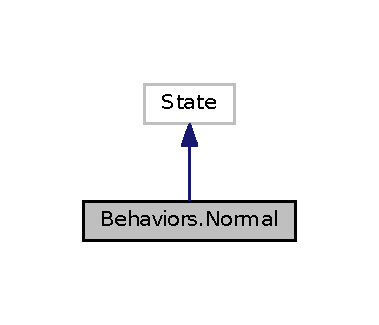
\includegraphics[width=182pt]{classBehaviors_1_1Normal__coll__graph}
\end{center}
\end{figure}
\subsection*{Public Member Functions}
\begin{DoxyCompactItemize}
\item 
def \hyperlink{classBehaviors_1_1Normal_a0d48c743470e9356c7eec875add25d1d}{\+\_\+\+\_\+init\+\_\+\+\_\+} (self)
\item 
def \hyperlink{classBehaviors_1_1Normal_ad85b58cb3f66b79ca64036abf251d191}{execute} (self, userdata)
\end{DoxyCompactItemize}


\subsection{Detailed Description}
\hyperlink{classBehaviors_1_1Normal}{Normal}\+: class that describes the \hyperlink{classBehaviors_1_1Normal}{Normal} state. 

\subsection{Constructor \& Destructor Documentation}
\index{Behaviors\+::\+Normal@{Behaviors\+::\+Normal}!\+\_\+\+\_\+init\+\_\+\+\_\+@{\+\_\+\+\_\+init\+\_\+\+\_\+}}
\index{\+\_\+\+\_\+init\+\_\+\+\_\+@{\+\_\+\+\_\+init\+\_\+\+\_\+}!Behaviors\+::\+Normal@{Behaviors\+::\+Normal}}
\subsubsection[{\texorpdfstring{\+\_\+\+\_\+init\+\_\+\+\_\+(self)}{__init__(self)}}]{\setlength{\rightskip}{0pt plus 5cm}def Behaviors.\+Normal.\+\_\+\+\_\+init\+\_\+\+\_\+ (
\begin{DoxyParamCaption}
\item[{}]{self}
\end{DoxyParamCaption}
)}\hypertarget{classBehaviors_1_1Normal_a0d48c743470e9356c7eec875add25d1d}{}\label{classBehaviors_1_1Normal_a0d48c743470e9356c7eec875add25d1d}


\subsection{Member Function Documentation}
\index{Behaviors\+::\+Normal@{Behaviors\+::\+Normal}!execute@{execute}}
\index{execute@{execute}!Behaviors\+::\+Normal@{Behaviors\+::\+Normal}}
\subsubsection[{\texorpdfstring{execute(self, userdata)}{execute(self, userdata)}}]{\setlength{\rightskip}{0pt plus 5cm}def Behaviors.\+Normal.\+execute (
\begin{DoxyParamCaption}
\item[{}]{self, }
\item[{}]{userdata}
\end{DoxyParamCaption}
)}\hypertarget{classBehaviors_1_1Normal_ad85b58cb3f66b79ca64036abf251d191}{}\label{classBehaviors_1_1Normal_ad85b58cb3f66b79ca64036abf251d191}


The documentation for this class was generated from the following file\+:\begin{DoxyCompactItemize}
\item 
exp\+\_\+assignment3/scripts/\hyperlink{Behaviors_8py}{Behaviors.\+py}\end{DoxyCompactItemize}

\hypertarget{classBehaviors_1_1Play}{}\section{Behaviors.\+Play Class Reference}
\label{classBehaviors_1_1Play}\index{Behaviors.\+Play@{Behaviors.\+Play}}


\hyperlink{classBehaviors_1_1Play}{Play}\+: class that describes the \hyperlink{classBehaviors_1_1Play}{Play} state.  




Inheritance diagram for Behaviors.\+Play\+:\nopagebreak
\begin{figure}[H]
\begin{center}
\leavevmode
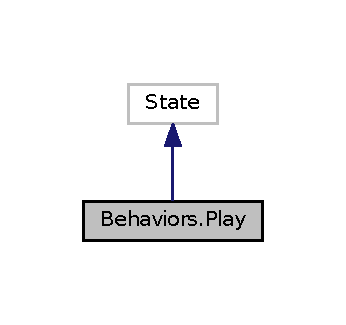
\includegraphics[width=166pt]{classBehaviors_1_1Play__inherit__graph}
\end{center}
\end{figure}


Collaboration diagram for Behaviors.\+Play\+:\nopagebreak
\begin{figure}[H]
\begin{center}
\leavevmode
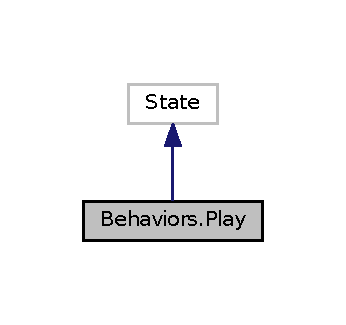
\includegraphics[width=166pt]{classBehaviors_1_1Play__coll__graph}
\end{center}
\end{figure}
\subsection*{Public Member Functions}
\begin{DoxyCompactItemize}
\item 
def {\bfseries \+\_\+\+\_\+init\+\_\+\+\_\+} (self)\hypertarget{classBehaviors_1_1Play_a5a5684ee3c87670a8eeeadb57ecba0d3}{}\label{classBehaviors_1_1Play_a5a5684ee3c87670a8eeeadb57ecba0d3}

\item 
def {\bfseries execute} (self, userdata)\hypertarget{classBehaviors_1_1Play_a2c8c1be112cceeb3b11c2450755306fe}{}\label{classBehaviors_1_1Play_a2c8c1be112cceeb3b11c2450755306fe}

\end{DoxyCompactItemize}


\subsection{Detailed Description}
\hyperlink{classBehaviors_1_1Play}{Play}\+: class that describes the \hyperlink{classBehaviors_1_1Play}{Play} state. 

The documentation for this class was generated from the following file\+:\begin{DoxyCompactItemize}
\item 
exp\+\_\+assignment3/scripts/Behaviors.\+py\end{DoxyCompactItemize}

\hypertarget{classBehaviors_1_1Recovery}{}\section{Behaviors.\+Recovery Class Reference}
\label{classBehaviors_1_1Recovery}\index{Behaviors.\+Recovery@{Behaviors.\+Recovery}}


\hyperlink{classBehaviors_1_1Recovery}{Recovery}\+: class that describes the \hyperlink{classBehaviors_1_1Recovery}{Recovery} state.  




Inheritance diagram for Behaviors.\+Recovery\+:\nopagebreak
\begin{figure}[H]
\begin{center}
\leavevmode
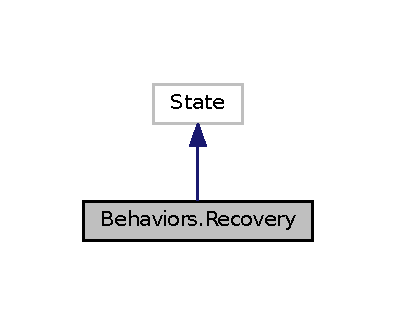
\includegraphics[width=190pt]{classBehaviors_1_1Recovery__inherit__graph}
\end{center}
\end{figure}


Collaboration diagram for Behaviors.\+Recovery\+:\nopagebreak
\begin{figure}[H]
\begin{center}
\leavevmode
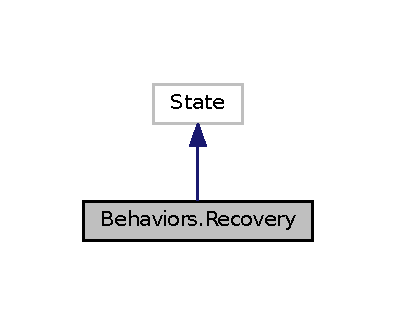
\includegraphics[width=190pt]{classBehaviors_1_1Recovery__coll__graph}
\end{center}
\end{figure}
\subsection*{Public Member Functions}
\begin{DoxyCompactItemize}
\item 
def \hyperlink{classBehaviors_1_1Recovery_a9952b507236ae466b701935a6e2482d6}{\+\_\+\+\_\+init\+\_\+\+\_\+} (self)
\item 
def \hyperlink{classBehaviors_1_1Recovery_a83ad65d2d9ca8efabb0c9977c8b8449a}{execute} (self, userdata)
\end{DoxyCompactItemize}


\subsection{Detailed Description}
\hyperlink{classBehaviors_1_1Recovery}{Recovery}\+: class that describes the \hyperlink{classBehaviors_1_1Recovery}{Recovery} state. 

\subsection{Constructor \& Destructor Documentation}
\index{Behaviors\+::\+Recovery@{Behaviors\+::\+Recovery}!\+\_\+\+\_\+init\+\_\+\+\_\+@{\+\_\+\+\_\+init\+\_\+\+\_\+}}
\index{\+\_\+\+\_\+init\+\_\+\+\_\+@{\+\_\+\+\_\+init\+\_\+\+\_\+}!Behaviors\+::\+Recovery@{Behaviors\+::\+Recovery}}
\subsubsection[{\texorpdfstring{\+\_\+\+\_\+init\+\_\+\+\_\+(self)}{__init__(self)}}]{\setlength{\rightskip}{0pt plus 5cm}def Behaviors.\+Recovery.\+\_\+\+\_\+init\+\_\+\+\_\+ (
\begin{DoxyParamCaption}
\item[{}]{self}
\end{DoxyParamCaption}
)}\hypertarget{classBehaviors_1_1Recovery_a9952b507236ae466b701935a6e2482d6}{}\label{classBehaviors_1_1Recovery_a9952b507236ae466b701935a6e2482d6}


\subsection{Member Function Documentation}
\index{Behaviors\+::\+Recovery@{Behaviors\+::\+Recovery}!execute@{execute}}
\index{execute@{execute}!Behaviors\+::\+Recovery@{Behaviors\+::\+Recovery}}
\subsubsection[{\texorpdfstring{execute(self, userdata)}{execute(self, userdata)}}]{\setlength{\rightskip}{0pt plus 5cm}def Behaviors.\+Recovery.\+execute (
\begin{DoxyParamCaption}
\item[{}]{self, }
\item[{}]{userdata}
\end{DoxyParamCaption}
)}\hypertarget{classBehaviors_1_1Recovery_a83ad65d2d9ca8efabb0c9977c8b8449a}{}\label{classBehaviors_1_1Recovery_a83ad65d2d9ca8efabb0c9977c8b8449a}


The documentation for this class was generated from the following file\+:\begin{DoxyCompactItemize}
\item 
exp\+\_\+assignment3/scripts/\hyperlink{Behaviors_8py}{Behaviors.\+py}\end{DoxyCompactItemize}

\hypertarget{classSlamGMappingNodelet}{}\section{Slam\+G\+Mapping\+Nodelet Class Reference}
\label{classSlamGMappingNodelet}\index{Slam\+G\+Mapping\+Nodelet@{Slam\+G\+Mapping\+Nodelet}}


Inheritance diagram for Slam\+G\+Mapping\+Nodelet\+:\nopagebreak
\begin{figure}[H]
\begin{center}
\leavevmode
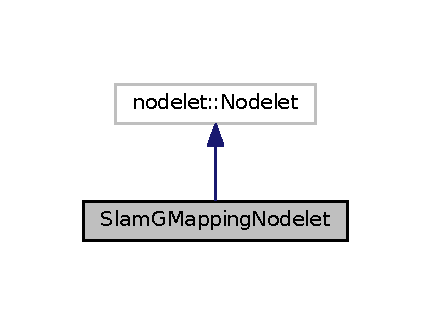
\includegraphics[width=207pt]{classSlamGMappingNodelet__inherit__graph}
\end{center}
\end{figure}


Collaboration diagram for Slam\+G\+Mapping\+Nodelet\+:\nopagebreak
\begin{figure}[H]
\begin{center}
\leavevmode
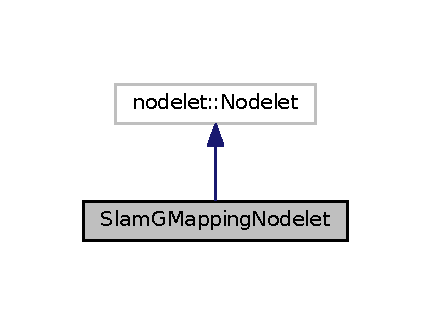
\includegraphics[width=207pt]{classSlamGMappingNodelet__coll__graph}
\end{center}
\end{figure}
\subsection*{Public Member Functions}
\begin{DoxyCompactItemize}
\item 
\hyperlink{classSlamGMappingNodelet_a32123727740dda66cf9f9905dc292015}{Slam\+G\+Mapping\+Nodelet} ()
\item 
\hyperlink{classSlamGMappingNodelet_a194f2f816307faf96427dc77c302c89a}{$\sim$\+Slam\+G\+Mapping\+Nodelet} ()
\item 
virtual void \hyperlink{classSlamGMappingNodelet_afeec962f825e389b6a52cd7f9debf425}{on\+Init} ()
\end{DoxyCompactItemize}


\subsection{Constructor \& Destructor Documentation}
\index{Slam\+G\+Mapping\+Nodelet@{Slam\+G\+Mapping\+Nodelet}!Slam\+G\+Mapping\+Nodelet@{Slam\+G\+Mapping\+Nodelet}}
\index{Slam\+G\+Mapping\+Nodelet@{Slam\+G\+Mapping\+Nodelet}!Slam\+G\+Mapping\+Nodelet@{Slam\+G\+Mapping\+Nodelet}}
\subsubsection[{\texorpdfstring{Slam\+G\+Mapping\+Nodelet()}{SlamGMappingNodelet()}}]{\setlength{\rightskip}{0pt plus 5cm}Slam\+G\+Mapping\+Nodelet\+::\+Slam\+G\+Mapping\+Nodelet (
\begin{DoxyParamCaption}
{}
\end{DoxyParamCaption}
)\hspace{0.3cm}{\ttfamily [inline]}}\hypertarget{classSlamGMappingNodelet_a32123727740dda66cf9f9905dc292015}{}\label{classSlamGMappingNodelet_a32123727740dda66cf9f9905dc292015}
\index{Slam\+G\+Mapping\+Nodelet@{Slam\+G\+Mapping\+Nodelet}!````~Slam\+G\+Mapping\+Nodelet@{$\sim$\+Slam\+G\+Mapping\+Nodelet}}
\index{````~Slam\+G\+Mapping\+Nodelet@{$\sim$\+Slam\+G\+Mapping\+Nodelet}!Slam\+G\+Mapping\+Nodelet@{Slam\+G\+Mapping\+Nodelet}}
\subsubsection[{\texorpdfstring{$\sim$\+Slam\+G\+Mapping\+Nodelet()}{~SlamGMappingNodelet()}}]{\setlength{\rightskip}{0pt plus 5cm}Slam\+G\+Mapping\+Nodelet\+::$\sim$\+Slam\+G\+Mapping\+Nodelet (
\begin{DoxyParamCaption}
{}
\end{DoxyParamCaption}
)\hspace{0.3cm}{\ttfamily [inline]}}\hypertarget{classSlamGMappingNodelet_a194f2f816307faf96427dc77c302c89a}{}\label{classSlamGMappingNodelet_a194f2f816307faf96427dc77c302c89a}


\subsection{Member Function Documentation}
\index{Slam\+G\+Mapping\+Nodelet@{Slam\+G\+Mapping\+Nodelet}!on\+Init@{on\+Init}}
\index{on\+Init@{on\+Init}!Slam\+G\+Mapping\+Nodelet@{Slam\+G\+Mapping\+Nodelet}}
\subsubsection[{\texorpdfstring{on\+Init()}{onInit()}}]{\setlength{\rightskip}{0pt plus 5cm}virtual void Slam\+G\+Mapping\+Nodelet\+::on\+Init (
\begin{DoxyParamCaption}
{}
\end{DoxyParamCaption}
)\hspace{0.3cm}{\ttfamily [inline]}, {\ttfamily [virtual]}}\hypertarget{classSlamGMappingNodelet_afeec962f825e389b6a52cd7f9debf425}{}\label{classSlamGMappingNodelet_afeec962f825e389b6a52cd7f9debf425}


The documentation for this class was generated from the following file\+:\begin{DoxyCompactItemize}
\item 
exp\+\_\+assignment3/src/\hyperlink{nodelet_8cpp}{nodelet.\+cpp}\end{DoxyCompactItemize}

\hypertarget{classBehaviors_1_1Sleep}{}\section{Behaviors.\+Sleep Class Reference}
\label{classBehaviors_1_1Sleep}\index{Behaviors.\+Sleep@{Behaviors.\+Sleep}}


\hyperlink{classBehaviors_1_1Sleep}{Sleep}\+: class that describes the \hyperlink{classBehaviors_1_1Sleep}{Sleep} state.  




Inheritance diagram for Behaviors.\+Sleep\+:\nopagebreak
\begin{figure}[H]
\begin{center}
\leavevmode
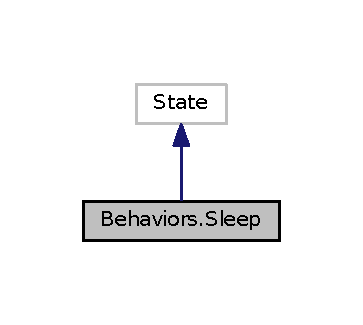
\includegraphics[width=174pt]{classBehaviors_1_1Sleep__inherit__graph}
\end{center}
\end{figure}


Collaboration diagram for Behaviors.\+Sleep\+:\nopagebreak
\begin{figure}[H]
\begin{center}
\leavevmode
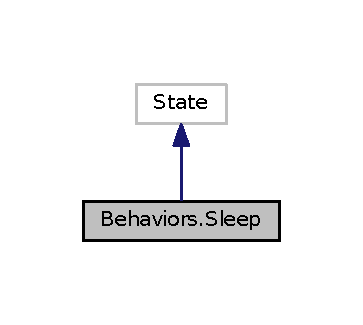
\includegraphics[width=174pt]{classBehaviors_1_1Sleep__coll__graph}
\end{center}
\end{figure}
\subsection*{Public Member Functions}
\begin{DoxyCompactItemize}
\item 
def \hyperlink{classBehaviors_1_1Sleep_accfb4124bccdbacf41004911ab15b447}{\+\_\+\+\_\+init\+\_\+\+\_\+} (self)
\item 
def \hyperlink{classBehaviors_1_1Sleep_ae2eb72a6c74a0c9154e7917550fafae4}{execute} (self, userdata)
\end{DoxyCompactItemize}


\subsection{Detailed Description}
\hyperlink{classBehaviors_1_1Sleep}{Sleep}\+: class that describes the \hyperlink{classBehaviors_1_1Sleep}{Sleep} state. 

\subsection{Constructor \& Destructor Documentation}
\index{Behaviors\+::\+Sleep@{Behaviors\+::\+Sleep}!\+\_\+\+\_\+init\+\_\+\+\_\+@{\+\_\+\+\_\+init\+\_\+\+\_\+}}
\index{\+\_\+\+\_\+init\+\_\+\+\_\+@{\+\_\+\+\_\+init\+\_\+\+\_\+}!Behaviors\+::\+Sleep@{Behaviors\+::\+Sleep}}
\subsubsection[{\texorpdfstring{\+\_\+\+\_\+init\+\_\+\+\_\+(self)}{__init__(self)}}]{\setlength{\rightskip}{0pt plus 5cm}def Behaviors.\+Sleep.\+\_\+\+\_\+init\+\_\+\+\_\+ (
\begin{DoxyParamCaption}
\item[{}]{self}
\end{DoxyParamCaption}
)}\hypertarget{classBehaviors_1_1Sleep_accfb4124bccdbacf41004911ab15b447}{}\label{classBehaviors_1_1Sleep_accfb4124bccdbacf41004911ab15b447}


\subsection{Member Function Documentation}
\index{Behaviors\+::\+Sleep@{Behaviors\+::\+Sleep}!execute@{execute}}
\index{execute@{execute}!Behaviors\+::\+Sleep@{Behaviors\+::\+Sleep}}
\subsubsection[{\texorpdfstring{execute(self, userdata)}{execute(self, userdata)}}]{\setlength{\rightskip}{0pt plus 5cm}def Behaviors.\+Sleep.\+execute (
\begin{DoxyParamCaption}
\item[{}]{self, }
\item[{}]{userdata}
\end{DoxyParamCaption}
)}\hypertarget{classBehaviors_1_1Sleep_ae2eb72a6c74a0c9154e7917550fafae4}{}\label{classBehaviors_1_1Sleep_ae2eb72a6c74a0c9154e7917550fafae4}


The documentation for this class was generated from the following file\+:\begin{DoxyCompactItemize}
\item 
exp\+\_\+assignment3/scripts/\hyperlink{Behaviors_8py}{Behaviors.\+py}\end{DoxyCompactItemize}

\hypertarget{classBehaviors_1_1Track}{}\section{Behaviors.\+Track Class Reference}
\label{classBehaviors_1_1Track}\index{Behaviors.\+Track@{Behaviors.\+Track}}


\hyperlink{classBehaviors_1_1Track}{Track}\+: class that describes the \hyperlink{classBehaviors_1_1Track}{Track} state.  




Inheritance diagram for Behaviors.\+Track\+:\nopagebreak
\begin{figure}[H]
\begin{center}
\leavevmode
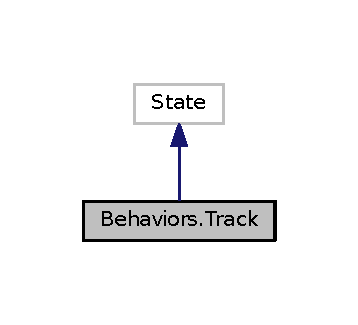
\includegraphics[width=172pt]{classBehaviors_1_1Track__inherit__graph}
\end{center}
\end{figure}


Collaboration diagram for Behaviors.\+Track\+:\nopagebreak
\begin{figure}[H]
\begin{center}
\leavevmode
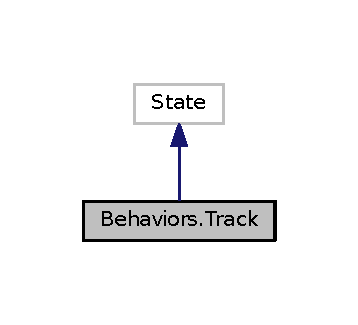
\includegraphics[width=172pt]{classBehaviors_1_1Track__coll__graph}
\end{center}
\end{figure}
\subsection*{Public Member Functions}
\begin{DoxyCompactItemize}
\item 
def \hyperlink{classBehaviors_1_1Track_ad4b822d13b3152463dfae09b7857cafe}{\+\_\+\+\_\+init\+\_\+\+\_\+} (self)
\item 
def \hyperlink{classBehaviors_1_1Track_a35b652d080f4b24379d06d0875c60658}{execute} (self, userdata)
\end{DoxyCompactItemize}


\subsection{Detailed Description}
\hyperlink{classBehaviors_1_1Track}{Track}\+: class that describes the \hyperlink{classBehaviors_1_1Track}{Track} state. 

\subsection{Constructor \& Destructor Documentation}
\index{Behaviors\+::\+Track@{Behaviors\+::\+Track}!\+\_\+\+\_\+init\+\_\+\+\_\+@{\+\_\+\+\_\+init\+\_\+\+\_\+}}
\index{\+\_\+\+\_\+init\+\_\+\+\_\+@{\+\_\+\+\_\+init\+\_\+\+\_\+}!Behaviors\+::\+Track@{Behaviors\+::\+Track}}
\subsubsection[{\texorpdfstring{\+\_\+\+\_\+init\+\_\+\+\_\+(self)}{__init__(self)}}]{\setlength{\rightskip}{0pt plus 5cm}def Behaviors.\+Track.\+\_\+\+\_\+init\+\_\+\+\_\+ (
\begin{DoxyParamCaption}
\item[{}]{self}
\end{DoxyParamCaption}
)}\hypertarget{classBehaviors_1_1Track_ad4b822d13b3152463dfae09b7857cafe}{}\label{classBehaviors_1_1Track_ad4b822d13b3152463dfae09b7857cafe}


\subsection{Member Function Documentation}
\index{Behaviors\+::\+Track@{Behaviors\+::\+Track}!execute@{execute}}
\index{execute@{execute}!Behaviors\+::\+Track@{Behaviors\+::\+Track}}
\subsubsection[{\texorpdfstring{execute(self, userdata)}{execute(self, userdata)}}]{\setlength{\rightskip}{0pt plus 5cm}def Behaviors.\+Track.\+execute (
\begin{DoxyParamCaption}
\item[{}]{self, }
\item[{}]{userdata}
\end{DoxyParamCaption}
)}\hypertarget{classBehaviors_1_1Track_a35b652d080f4b24379d06d0875c60658}{}\label{classBehaviors_1_1Track_a35b652d080f4b24379d06d0875c60658}


The documentation for this class was generated from the following file\+:\begin{DoxyCompactItemize}
\item 
exp\+\_\+assignment3/scripts/\hyperlink{Behaviors_8py}{Behaviors.\+py}\end{DoxyCompactItemize}

%--- End generated contents ---

% Index
\backmatter
\newpage
\phantomsection
\clearemptydoublepage
\addcontentsline{toc}{chapter}{Index}
\printindex

\end{document}
